\documentclass[12pt, a4paper]{article}

% Standard packages for economics papers
\usepackage[utf8]{inputenc}
\usepackage[T1]{fontenc}
\usepackage{geometry}
\geometry{a4paper, margin=1in}
\usepackage{setspace}
\onehalfspacing % Common for readability; use \doublespacing if submitting for review
\usepackage{amsmath, amssymb, amsthm}
\usepackage{graphicx}
\usepackage{booktabs}  % Creates beautiful top/mid/bottom rules instead of ugly grids
\usepackage{multirow}  % Allows the p0 values to span across the T rows seamlessly
\usepackage{rotating}  % Allows for sideways tables (sidewaystable)
\usepackage{caption}
\usepackage{subcaption}
\usepackage[colorlinks=true, linkcolor=blue, citecolor=blue, urlcolor=blue]{hyperref}

% BibLaTeX setup for Zotero Better BibLaTeX
\usepackage[style=authoryear, backend=biber, natbib=true, maxcitenames=2]{biblatex}
\addbibresource{Monte Carlo Simulations.bib}

% Title and Author Information
\title{Embracing Lag Uncertainty: Bayesian Model Averaging in Set-Identifed Structural VARs}
\author{
    Ak\i n Ayd\i n\thanks{Ludwig-Maximilian University of Munich, \href{mailto:akin.aydin@campus.lmu.de}{akin.aydin@campus.lmu.de}} \and
    Ferdinand Loser\thanks{Ludwig-Maximilian University of Munich, \href{mailto:ferdinand.loser@campus.lmu.de}{ferdinand.loser@campus.lmu.de}}
}
\date{\today \\ \vspace{0.5cm} \textit{Seminar Evaluating Econometric Methods using Monte Carlo Simulations }(Prof. Derya Uysal)}

\begin{document}

\maketitle

\begin{abstract}
\noindent
This is the abstract for your paper. Briefly state the purpose of the research, the principal results, and major conclusions. The abstract should be self-contained and citation-free.
\vspace{1em}\\
\noindent\textbf{Keywords:} Structural Vector Autoregression (SVAR), Set Identification, Bayesian Model Averaging (BMA), Model Uncertainty, Lag Order Selection, Monte Carlo Simulation \\
\noindent\textbf{JEL Codes:} C11, C15, C32, C52 % Update with relevant JEL classification codes
\end{abstract}

\newpage

\section{Introduction}
\label{sec:introduction}
Introduce the problem of lag selection and parameter proliferation in Structural VARs. Highlight the debate between hard lag selection (Information Criteria) and Bayesian methods (Shrinkage and Model Averaging).

\section{Simulation Design}
\label{sec:methodology}

This Monte Carlo simulation study follows \citet{ivanovPractitionersGuideLag2005} design with several alterations in order to make our extensions feasible and to fit the needs of our analysis. First of all, we only use one monthly DGP based on the empirical VAR study of \citet{kilianRoleInventoriesSpeculative2014}. Therefore, we do not get estimations for quarterly VAR series or VEC series, and additionally, we do not have additional robustness by including several different series with different macroeconomic indicators and movements. The main reason for this is our tight time constraint. However, this concern is also not to be overstated as \citet{ivanovPractitionersGuideLag2005} did not find big differences between different DGPs of the same type (monthly, quarterly, VEC). We use the dataset from \citet{kilianRoleInventoriesSpeculative2014} containing the following 4 variables: percent change in global oil production, real activity index from \citet{kilianNotAllOil2009}, the log real price of oil, and changes in OECD crude oil inventories. Just as in the original study, we first estimate a VAR with a set lag order of these 4 variables and then use the sign restrictions approach explained earlier to identify structural IRFs. Therefore, our estimation becomes much more complex and updates the findings of \citet{ivanovPractitionersGuideLag2005} to a more modern and widely used approach in the literature. All papers used for the DGP generation in \citet{ivanovPractitionersGuideLag2005} are from the 1990s and early 2000s and are based on the Cholesky decomposition approach for identification. Cholesky decomposition only gives one unique set of IRFs, whereas the sign restrictions approach principally has an infinite number of possible sets of IRFs. 

We follow \citet{kilianRoleInventoriesSpeculative2014} in searching for a large number of admissible IRFs by randomly drawing from the space of rotation matrices. We use exactly the same sign restriction matrix, but limit the number of periods for which dynamic sign restrictions are imposed to 3 instead of 12, and do not include additional elasticity bounds. This is a significant diversion from the original study as it makes the identification more agnostic and opens up the space of admissible IRFs. We are therefore closer to the original sign restrictions approach of \citet{uhligWhatAreEffects2005}. We understand that the additional restrictions of \citet{kilianRoleInventoriesSpeculative2014} are motivated by limiting the set to fit theory and other empirical evidence, we have to take the less restrictive approach in order to make the estimation feasible. Especially for low lag orders and smaller samples, these restrictions have proven to be so strong that even several million draws of the rotation matrix do not give us enough admissible IRFs to make a good inference. For the simulation, this exceedingly high number of draws would need to then be repeated hundreds of times.

Out of this set, we select the median target IRF as our true IRF, which is defined as the IRF that has the smallest distance to the median of all admissible IRFs. The DGP follows this IRF as it is generated by a structural VAR model using the structural impact matrix $\tilde{B}$ that corresponds to the median target IRF as the parameter for the structural shocks $e_t$, which is drawn from an i.i.d. standard normal distribution. The formula for the DGP is represented by a structural VAR model using the estimated reduced form parameters $A$ (for the lag coefficients $y_{t-p}$) and $V$ (for the monthly dummy parameters $d_t$) and the structural impact matrix $\tilde{B}$ as follows:

\begin{equation}
    y_t = V d_t + A y_{t-p} + \tilde{B} e_t
\end{equation}

We estimate these parameters using the original data for five different lag orders, $p_0 \in {4,6,8,10}$ and create DGPs with different sample sizes, $T \in {240, 300, 360, 480, 600}$, where $T=N+\bar{p}$. $\bar{p}$ is the set of lag orders that are considered for both the IC and the BVAR estimations; it is uniformly set to $\bar{p}=12$ to ensure that the true lag order $p_0$ is part of the set. These specifications directly follow \citet{ivanovPractitionersGuideLag2005}. We do not increase the number of lags or higher sample sizes in order to keep the comparison intact and to keep computational capacities available for the switch to sign restriction decomposition and the addition of BVAR. For sampling, we use random draws of length $p_0$ from the original dataset as initial values, then apply the parametric bootstrap using the SVAR described above and generate sequences of lengths $T$.

On each of these samples, OLS VARs fitted by lag orders selected by both the three ICs as well as the BMA determined OLS VARs and BVARs, for both the geometric and BIC-based approach, are estimated, a fixed number of admissible IRFs found, and the median target IRF determined. We only include AIC, BIC and HQC as information criteria and omit the Likelihood Ratio tests and the Lagrange Multiplier test for lag selection as these have become practically irrelevant in the last 20 years for macroeconomic time series analysis and were also shown to perform poorly in \citet{ivanovPractitionersGuideLag2005}. The four different BMA estimations follow the methodology described in the previous section. The space of optimal shrinkage parameters for the implementation with BVAR is limited to $\lambda_1 \in \{0.05, 0.2, 0.35, 0.5, 0.65, 0.8, 0.95\}$ in order to make computation in the simulation feasible. It still captures a good range of typically used $lambda_1$-values, both tighter and looser specifications. 

Finally, the squared error matrix of the selected median target IRF to the true DGP IRF is calculated, collapsed into a scalar total squared error by summation. Then we estimate the ratio of this squared error of a specific estimation approach to the model fitted by the true lag order $p_0$. Therefore, the deviations of the true IRF are directly put into relation to how well a correctly specified model compares for the given sample. Finally, we estimate the MSE by calculating the geometric mean of these individual ratios. The geometric mean is preferred over the arithmetic mean as the ratios are bounded on the left side at 0, but unbounded on the right side. Outliers on the right side are hence overweighed in the arithmetic mean. The relative MSE for one method for one true lag order $p_0$ and one sample size $T$ is given by the following formula:

\begin{equation}
    MSE_{relative} = \exp\left( \frac{1}{n} \sum_{i=1}^{n} \ln(r_i) \right) \text{ where } r_i=\frac{TSE_i}{TSE^{p_0}_{i}}
\end{equation}

While, for a single estimation it is possible to estimate millions of admissible IRFs, the Monte Carlo simulation approach doesn't allow for such a large number of draws. In establishing the median target IRF specific to the DGP, we set the number of discovered admissible IRFs to 1 million so as to have a very accurate median target IRF for the specific dataset. In the Monte Carlo Simulation, we reduce this number drastically to 100 as it has proven to be the absolute limit that still allows us to have an acceptable number of Monte Carlo iterations, 1000, for our set of different methods. Even with computational optimization by parallel processing, more draws are not applicable under our hardware constraints. For each individual iteration, the median target IRF is therefore less accurately determined. However, because we use relative MSEs as our performance measure and repeat the process 1000 times, this should not impact the interpretability of our results. 

% Placing the MDD Surface here visually justifies your optimization approach.
\begin{figure}[htbp]
    \centering
    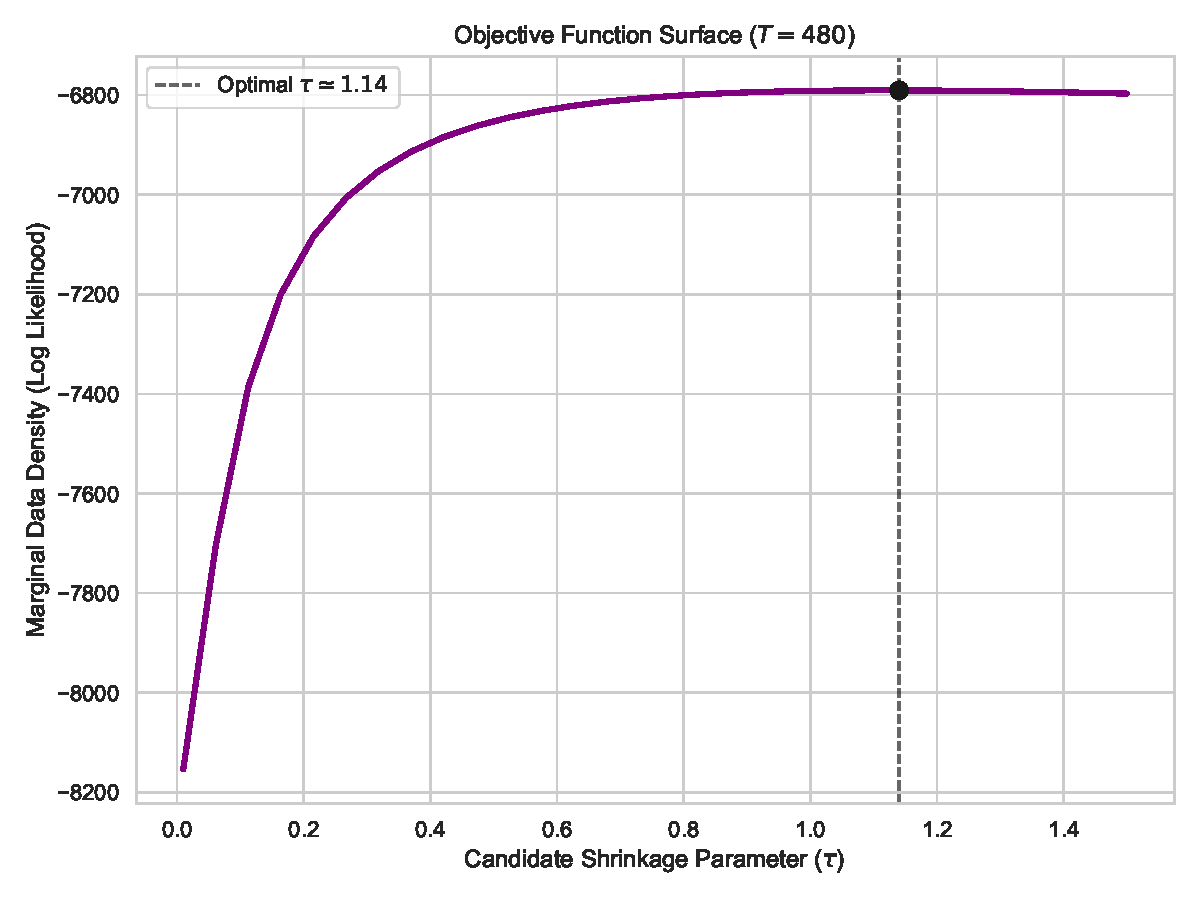
\includegraphics[width=0.85\textwidth]{Figures/Fig3_MDD_Surface.pdf}
    \caption{Objective Function Surface for Marginal Data Density Optimization. The peak represents the optimal balance between model fit and parameter penalty.}
    \label{fig:mdd_surface}
\end{figure}

\section{Results}
\label{sec:results}
Present the results of the Monte Carlo simulations, broken down by the specific strategies employed to handle model uncertainty.

\subsection{Behavior of Standard Information Criteria}
As established theoretically as well as in the foundational Monte Carlo simulation study on information criterias, \citet{lutkepohlComparisonCriteriaEstimating1985}, AIC tends to select higher lag orders than HQC and BIC, and BIC typically has the strongest reduction in included lags. Our results confirm this as seen in \ref{tab:ic_lag_orders}.

\begin{table}[htbp]
\centering
\caption{Average Evaluated Lag Order ($\hat{p}$) selected by Information Criteria.}
\label{tab:ic_lag_orders}
\begin{tabular}{llccc}
\toprule
 & Estimator & AIC & BIC & HQC \\
$p_0$ & $T$ &  &  &  \\
\midrule
\multirow[t]{2}{*}{4} & 240 & 2.99 & 1.95 & 2.06 \\
 & 600 & 3.80 & 2.02 & 2.66 \\
\multirow[t]{2}{*}{10} & 240 & 6.54 & 1.96 & 2.07 \\
 & 600 & 9.16 & 2.02 & 4.03 \\
\bottomrule
\end{tabular}
\end{table}


\subsection{The Uncertainty Strategy: Averaging vs. Selection}
Here, we evaluate True Bayesian Model Averaging (BMA) against Information Criteria. We focus on how BMA acts as an insurance policy against catastrophic lag misspecification in small samples.

\begin{sidewaystable}[htbp]
\centering
\caption{Relative Mean Squared Error: Hard Selection vs.~Bayesian Model Averaging.}
\label{tab:uncertainty_mse}
\begin{tabular}{llcccccc}
\toprule
 &  & AIC & SIC/BIC & HQC & \begin{tabular}{@{}c@{}}OLS BMA \\ (BIC-W)\end{tabular} & \begin{tabular}{@{}c@{}}BMA BVAR-WN \\ (BIC-W, $\tau=0.20$)\end{tabular} & \begin{tabular}{@{}c@{}}BMA BVAR-WN \\ (BIC-W, $\tau=0.50$)\end{tabular} \\
$T$ & $p_0$ &  &  &  &  &  &  \\
\midrule
\multirow[t]{4}{*}{96} & 4 & 1.921 & \bfseries 0.958 & 1.253 & 1.234 & 1.095 & 1.248 \\
 & 6 & 1.229 & 1.248 & 1.089 & 0.893 & \bfseries 0.822 & 1.039 \\
 & 8 & 1.813 & 1.298 & 1.287 & 1.113 & 1.170 & \bfseries 1.096 \\
 & 10 & 1.179 & 0.813 & 0.604 & 0.617 & 0.698 & \bfseries 0.538 \\
\multirow[t]{4}{*}{144} & 4 & 1.330 & 1.363 & 1.252 & 1.787 & \bfseries 1.231 & 1.484 \\
 & 6 & 1.181 & 0.689 & 0.756 & 0.983 & 0.686 & \bfseries 0.676 \\
 & 8 & \bfseries 0.672 & 1.333 & 0.755 & 0.841 & 1.072 & 0.903 \\
 & 10 & 0.556 & 0.824 & 0.793 & 1.050 & \bfseries 0.299 & 0.637 \\
\multirow[t]{4}{*}{240} & 4 & 0.701 & \bfseries 0.589 & 0.685 & 0.912 & 0.743 & 0.840 \\
 & 6 & 1.011 & 1.046 & 1.111 & \bfseries 0.789 & 0.944 & 0.817 \\
 & 8 & 1.177 & 1.372 & 1.416 & 1.095 & 1.006 & \bfseries 0.742 \\
 & 10 & 1.071 & 1.132 & 1.307 & \bfseries 0.981 & 1.154 & 1.636 \\
\multirow[t]{4}{*}{480} & 4 & \bfseries 1.091 & 2.121 & 2.015 & 1.373 & 2.100 & 1.435 \\
 & 6 & 0.688 & 0.762 & \bfseries 0.635 & 1.149 & 0.924 & 1.520 \\
 & 8 & 1.000 & 0.914 & 0.826 & 0.740 & \bfseries 0.527 & 0.755 \\
 & 10 & 1.340 & 1.042 & 1.005 & 0.994 & 1.671 & \bfseries 0.787 \\
\bottomrule
\end{tabular}
\end{sidewaystable}


\ref{tab:bma_posterior} and \ref{fig:bma_heatmaps_grid} reveal how the weights are spread out for the four different BMA methods. Both OLS-based approaches produce a much more concentrated weighting scheme as higher lag orders are completely eliminated due to their high parameter variance in OLS-estimation. High lag orders are found to still introduce too much variance into the estimation to suffice a non-zero weight. On the other hand, both BVAR-based approaches spread out the weights much wider, and do not set high lag orders to 0. The additional parameter shrinkage of the BVAR estimation therefore enables BMA to still include more lag orders as their parameters are further shrunk towards 0. This shrinkage is further adapted to the specific chosen lag order $p$ as both geometric and joint grid BMA jointly optimize $p$ and the $p$-specific $\lambda_1$-value. A higher lag-order can therefore be combined with a tighter $\lambda_1$-value in order to shrink down the higher lags more drastically. 

\ref{fig:tau_to_p} illustrates how smaller $\lambda_1$-values are selected for higher lag orders $p$.

\begin{table}[htbp]
\centering
\caption{Posterior Lag-Weight Distribution across all BMA architectures ($p_0 = 4$).}
\label{tab:bma_posterior}
\begin{tabular}{l|cccccccccccccccc}
\toprule
Estimator & OLS-BMA & OLS-Geom-BMA & Joint-BMA & Geom-BMA & OLS-BMA & OLS-Geom-BMA & Joint-BMA & Geom-BMA & OLS-BMA & OLS-Geom-BMA & Joint-BMA & Geom-BMA & OLS-BMA & OLS-Geom-BMA & Joint-BMA & Geom-BMA \\
$T$ & 96 & 96 & 96 & 96 & 144 & 144 & 144 & 144 & 240 & 240 & 240 & 240 & 480 & 480 & 480 & 480 \\
Statistic / Lag &  &  &  &  &  &  &  &  &  &  &  &  &  &  &  &  \\
\midrule
$E[p]$ & 1.24 & 1.22 & 7.01 & 3.39 & 1.41 & 1.38 & 5.07 & 3.01 & 1.96 & 1.95 & 4.41 & 3.23 & 2.00 & 2.00 & 3.92 & 3.46 \\
p=1 & 75.7\% & 77.6\% & 0.7\% & 4.3\% & 59.5\% & 62.4\% & 0.1\% & 1.1\% & 3.9\% & 4.7\% & - & - & - & - & - & - \\
p=2 & 24.3\% & 22.4\% & 11.1\% & 35.1\% & 40.5\% & 37.6\% & 20.1\% & 42.7\% & 96.1\% & 95.3\% & 12.9\% & 26.6\% & 100.0\% & 100.0\% & 8.4\% & 15.0\% \\
p=3 & - & - & 12.6\% & 27.4\% & - & - & 22.6\% & 31.7\% & - & - & 28.5\% & 40.3\% & - & - & 25.1\% & 33.0\% \\
p=4 & - & - & 8.6\% & 13.5\% & - & - & 13.3\% & 13.1\% & - & - & 23.0\% & 21.4\% & - & - & 47.3\% & 44.5\% \\
p=5 & - & - & 7.1\% & 7.8\% & - & - & 9.6\% & 6.0\% & - & - & 14.0\% & 8.1\% & - & - & 12.2\% & 6.4\% \\
p=6 & - & - & 6.2\% & 4.4\% & - & - & 7.2\% & 2.8\% & - & - & 7.8\% & 2.6\% & - & - & 4.0\% & 1.0\% \\
p=7 & - & - & 6.5\% & 2.8\% & - & - & 5.6\% & 1.4\% & - & - & 4.5\% & 0.7\% & - & - & 1.4\% & 0.1\% \\
p=8 & - & - & 6.5\% & 1.8\% & - & - & 4.3\% & 0.6\% & - & - & 2.8\% & 0.1\% & - & - & 0.6\% & - \\
p=9 & - & - & 7.6\% & 1.3\% & - & - & 4.1\% & 0.3\% & - & - & 2.0\% & - & - & - & 0.3\% & - \\
p=10 & - & - & 9.1\% & 0.8\% & - & - & 4.2\% & 0.2\% & - & - & 1.8\% & - & - & - & 0.3\% & - \\
p=11 & - & - & 11.0\% & 0.5\% & - & - & 4.5\% & - & - & - & 1.5\% & - & - & - & 0.3\% & - \\
p=12 & - & - & 13.0\% & 0.3\% & - & - & 4.4\% & - & - & - & 1.2\% & - & - & - & 0.2\% & - \\
\bottomrule
\end{tabular}
\end{table}


\begin{figure}[p] % The [p] tells LaTeX to put this on its own dedicated page
    \centering
    
    % Top Left: Figure 5
    \begin{subfigure}[b]{0.48\textwidth}
        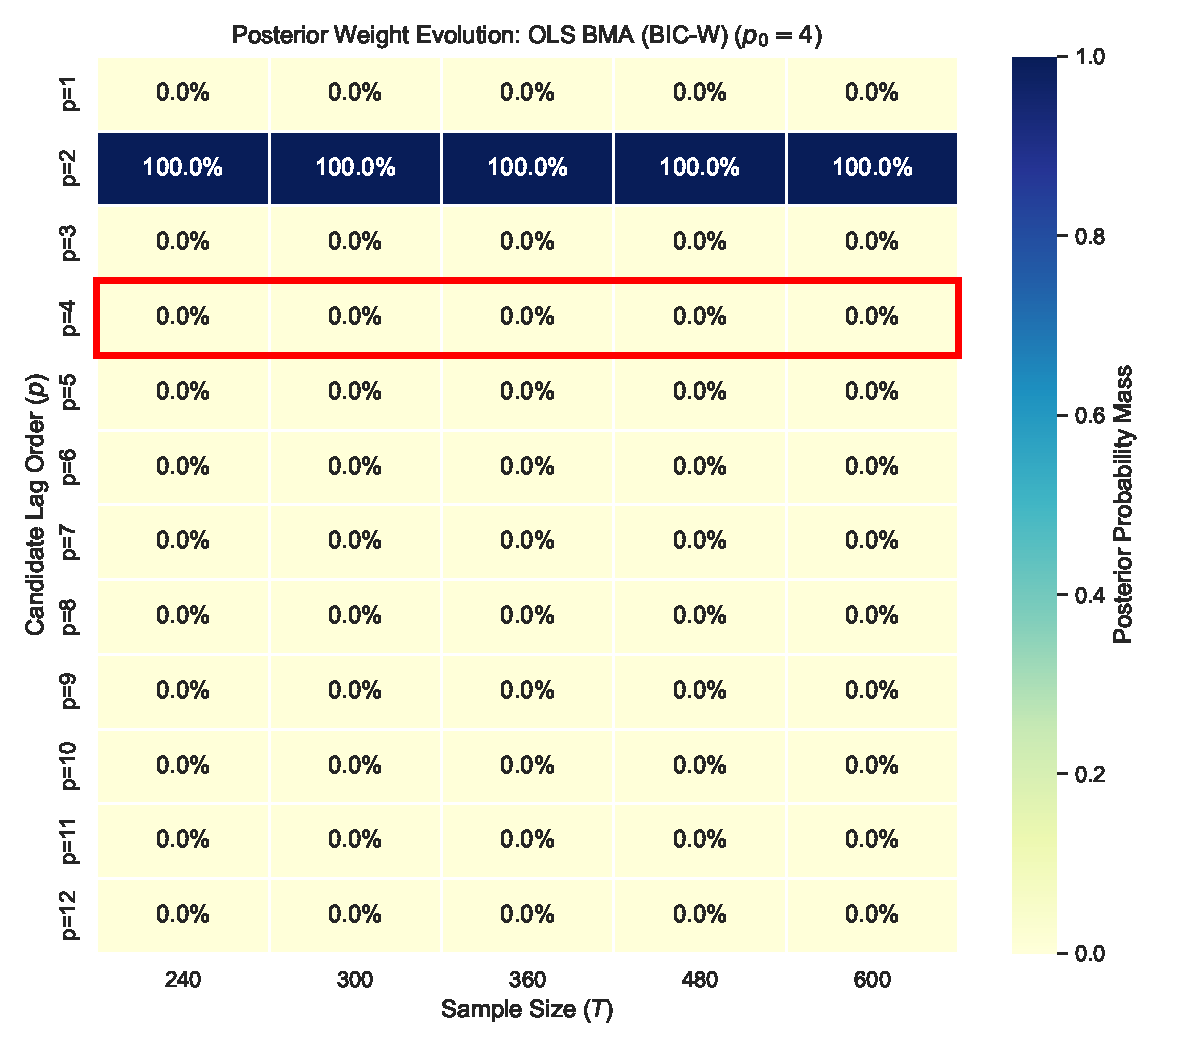
\includegraphics[width=\textwidth]{Figures/Fig5_BMA_Heatmap_OLS.pdf}
        \caption{OLS BMA (BIC-weighted)}
        \label{fig:heat_ols}
    \end{subfigure}
    \hfill % Adds horizontal space between the two columns
    % Top Right: Figure 6
    \begin{subfigure}[b]{0.48\textwidth}
        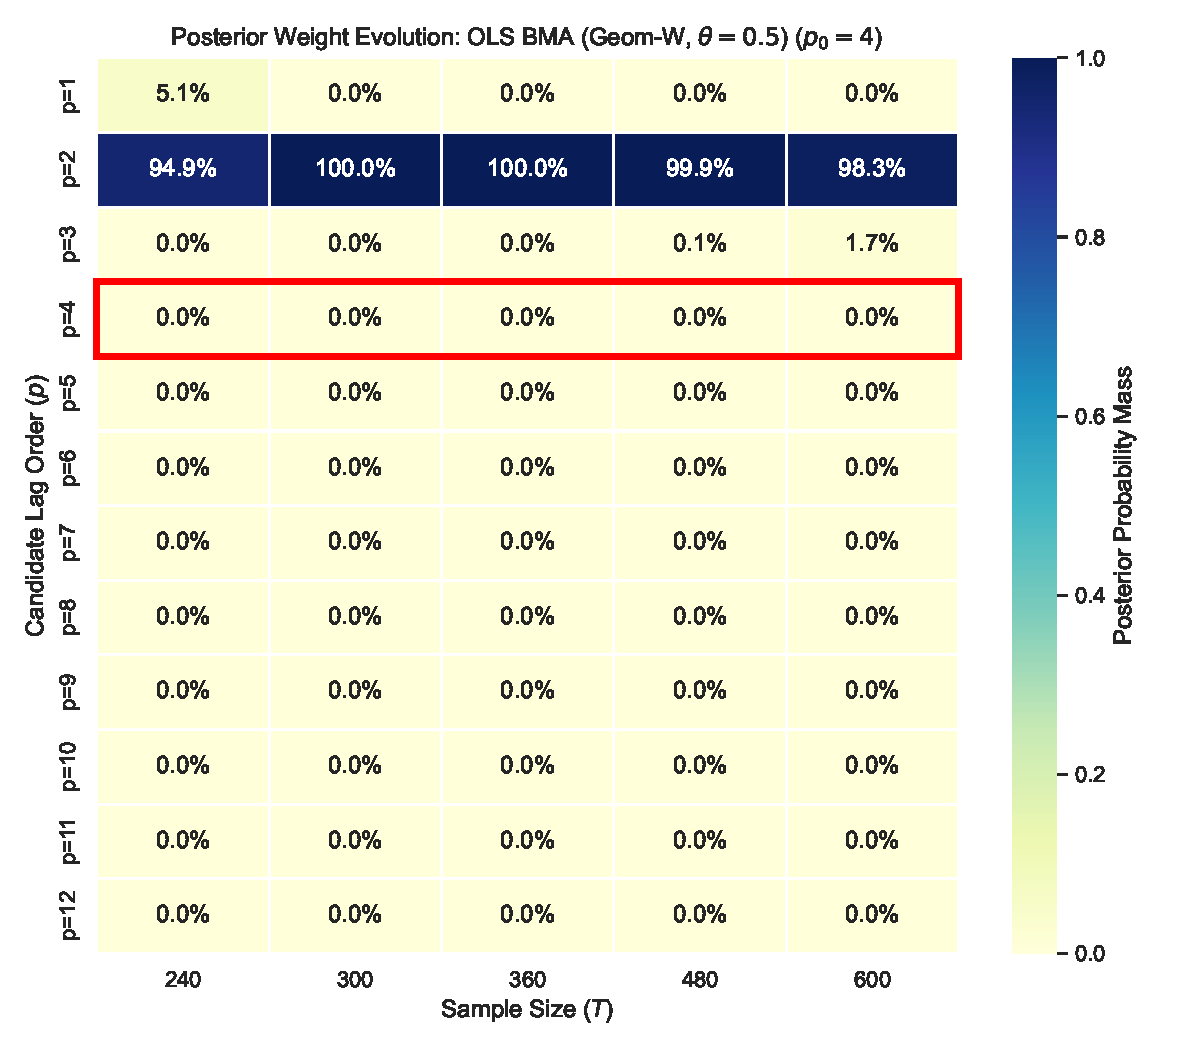
\includegraphics[width=\textwidth]{Figures/Fig6_BMA_Heatmap_OLS_Geom.pdf}
        \caption{OLS BMA (Geom. BIC-weighted, $\theta=0.5$)}
        \label{fig:heat_ols_geom}
    \end{subfigure}
    
    \vspace{2em} % Adds vertical space between the rows
    
    % Bottom Left: Figure 7
    \begin{subfigure}[b]{0.48\textwidth}
        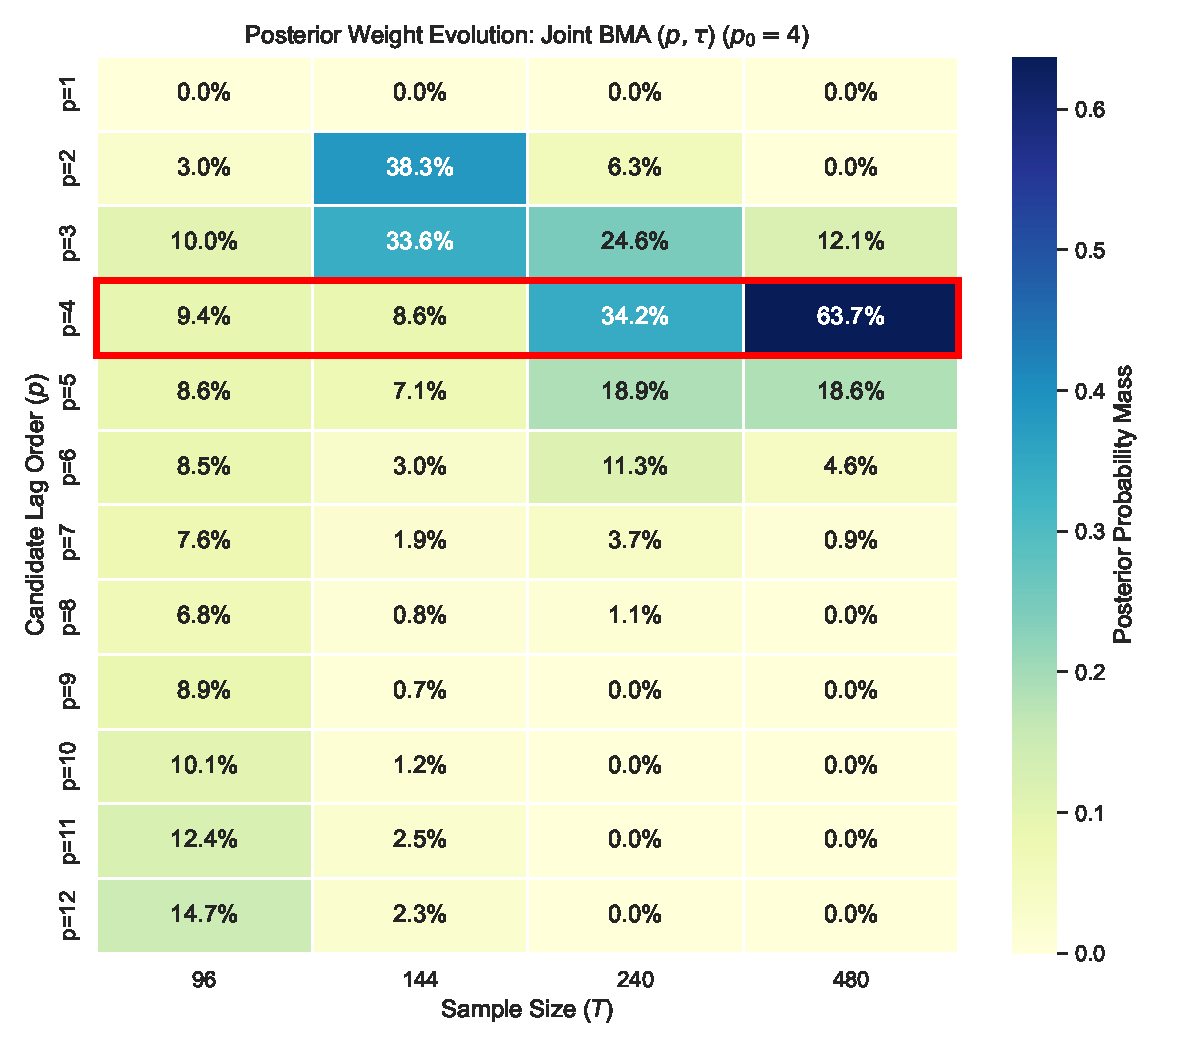
\includegraphics[width=\textwidth]{Figures/Fig7_BMA_Heatmap_Joint.pdf}
        \caption{Joint Grid BMA ($p, \tau$)}
        \label{fig:heat_joint}
    \end{subfigure}
    \hfill
    % Bottom Right: Figure 8
    \begin{subfigure}[b]{0.48\textwidth}
        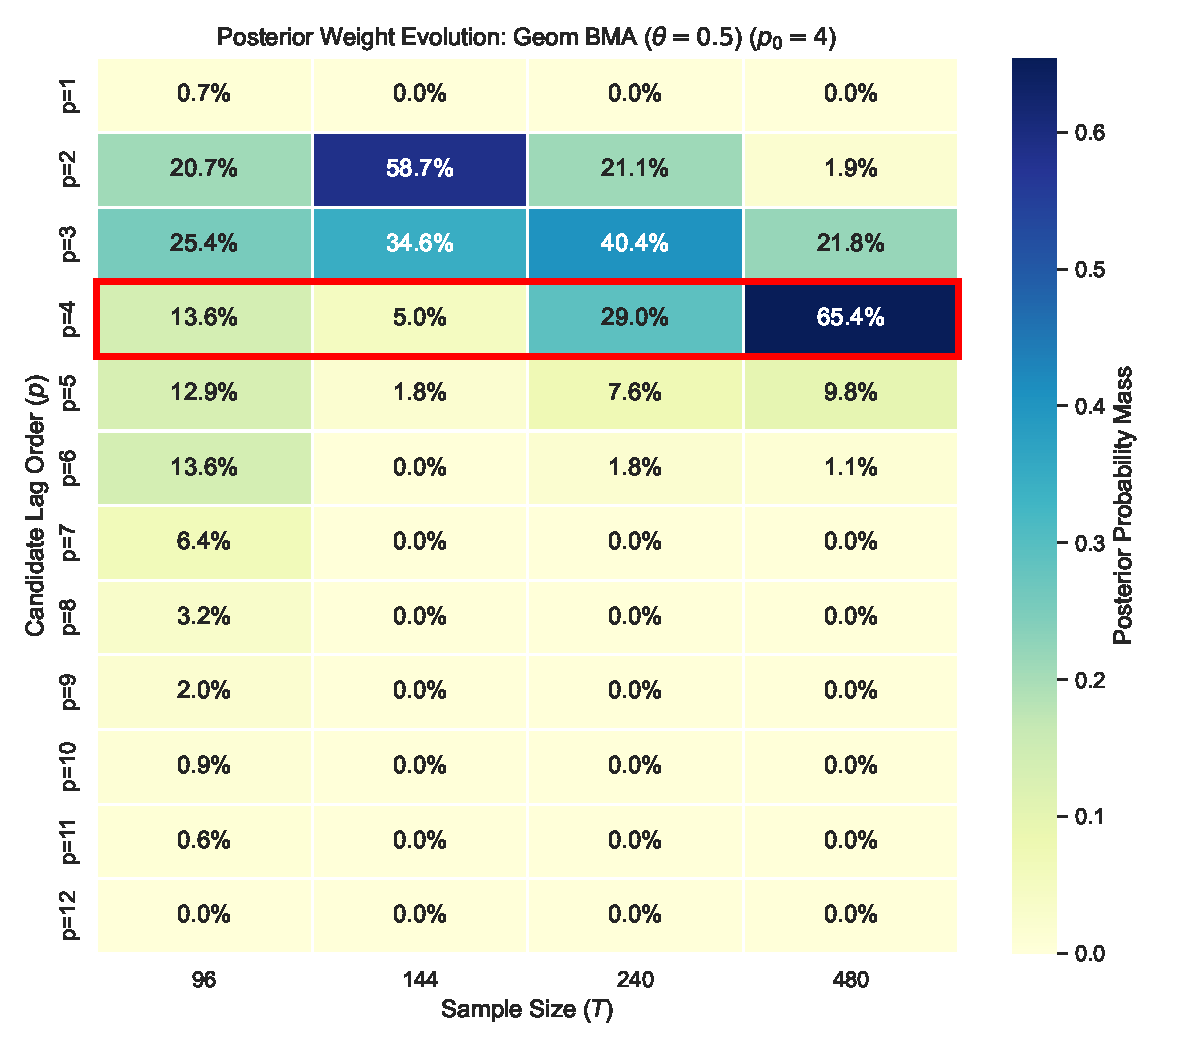
\includegraphics[width=\textwidth]{Figures/Fig8_BMA_Heatmap_Geom.pdf}
        \caption{Geometric Grid BMA ($\theta=0.5$)}
        \label{fig:heat_geom}
    \end{subfigure}
    
    \caption{Posterior Weight Evolution across all four BMA architectures ($p_0=4$).}
    \label{fig:bma_heatmaps_grid}
\end{figure}

\begin{figure}[htbp]
    \centering
    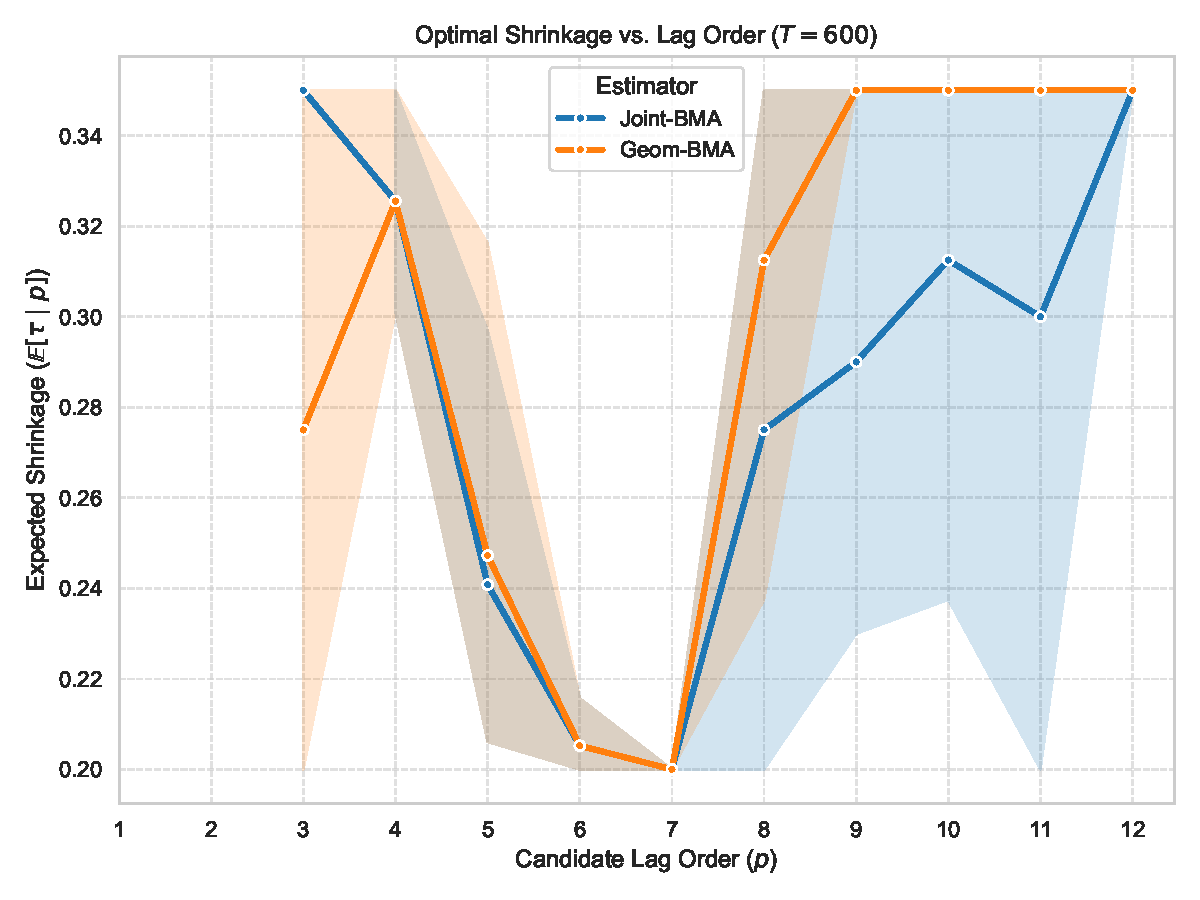
\includegraphics[width=0.85\textwidth]{Figures/Fig9_Tau_Comparison_T600.pdf}
    \caption{Optimal $lambda_1$ is adapted to the lag order $p$.}
    \label{fig:tau_to_p}
\end{figure}

\clearpage
\section{Conclusion}
\label{sec:conclusion}

Summarize the main findings, specifically highlighting how optimal $\tau$ selection and true BMA systematically outperform standard econometric heuristics in finite samples.

\newpage
% Print the bibliography
\section*{References}
\printbibliography

\section*{Declaration of AI Usage}

During the preparation of this seminar paper, I, [NAME], used Claude, Gemini, and ChatGPT for help with coding, research, and adapting writing to academic standards. I have reviewed and edited the content as needed and take full responsibility for the content.

[NAME]

\end{document}